\documentclass[aspectratio=169]{beamer}
% Shared Beamer style for this repository.
\usepackage[fontset=none]{ctex}
\usepackage{fontspec}
\setmainfont{DejaVu Serif}
\setsansfont{DejaVu Sans}
\setmonofont{DejaVu Sans Mono}
\setCJKmainfont{Noto Serif CJK SC}[BoldFont={Noto Serif CJK SC Bold}]
\setCJKsansfont{Noto Sans CJK SC}[BoldFont={Noto Sans CJK SC Bold}]
\setCJKmonofont{Noto Sans Mono CJK SC}

\usetheme{Madrid}
\usefonttheme{serif}
\setbeamertemplate{navigation symbols}{}
\setbeamertemplate{footline}[frame number]

\usepackage{graphicx}
\usepackage{amsmath,amssymb}
\usepackage{booktabs}
\usepackage{array}
\usepackage{xcolor}
\usepackage{listings}
\usepackage{tikz}
\usetikzlibrary{shapes,arrows,positioning}

% Color system
\definecolor{dcPrimary}{RGB}{21,101,117}
\definecolor{dcSecondary}{RGB}{140,115,72}
\definecolor{dcAccent}{RGB}{184,92,63}
\definecolor{dcMuted}{RGB}{230,250,252}
\definecolor{dcWarmBG}{RGB}{255,245,230}
\definecolor{dcCodeBG}{RGB}{247,248,250}
\definecolor{dcCodeFrame}{RGB}{200,210,215}

\setbeamercolor{structure}{fg=dcPrimary}
\setbeamercolor{palette primary}{fg=dcPrimary,bg=dcMuted}
\setbeamercolor{palette secondary}{fg=dcSecondary,bg=dcMuted!90}
\setbeamercolor{palette tertiary}{fg=dcPrimary,bg=dcMuted!80}
\setbeamercolor{frametitle}{fg=white,bg=dcPrimary}
\setbeamercolor{title}{fg=dcPrimary}
\setbeamercolor{alerted text}{fg=dcAccent}
\setbeamercolor{item}{fg=dcPrimary}
\setbeamercolor{subitem}{fg=dcSecondary}
\setbeamercolor{block title}{fg=white,bg=dcPrimary}
\setbeamercolor{block body}{bg=dcMuted}
\setbeamercolor{block title example}{fg=white,bg=dcSecondary}
\setbeamercolor{block body example}{bg=dcWarmBG}
\setbeamercolor{block title alerted}{fg=white,bg=dcAccent}
\setbeamercolor{block body alerted}{bg=dcWarmBG}
\setbeamercolor{footline}{fg=dcPrimary}

\lstset{
  basicstyle=\ttfamily\footnotesize,
  backgroundcolor=\color{dcCodeBG},
  frame=single,
  rulecolor=\color{dcCodeFrame},
  numbers=none,
  breaklines=true,
  showstringspaces=false,
  tabsize=2
}


\title{数字抽象、CMOS 与组合逻辑基础}
\subtitle{第三章第一讲：从 MOS 器件到逻辑门，再到组合逻辑与时间直觉}
\author{Digital Circuit Getting Started}
\date{\today}

\graphicspath{{figures/}}

\begin{document}

\begin{frame}
  \titlepage
\end{frame}

\begin{frame}{Learning Objectives}
\begin{itemize}
  \item 理解逻辑 0/1 不是天降符号，而是器件、电压阈值、噪声容限共同维持的工程抽象
  \item 建立 MOS、CMOS 反相器、NAND/NOR 与组合逻辑之间的递进关系
  \item 理解门延迟、fanout、transition 会沿路径耦合传播，时间问题从第一讲就已经出现
  \item 看懂组合逻辑中的竞争与冒险，并能用半加器把表达式、真值表和门级结构接起来
\end{itemize}
\end{frame}

\begin{frame}{The Game Plan}
\begin{enumerate}
  \item 为什么数字抽象在物理世界里成立
  \item MOS 管如何组成上拉 / 下拉网络
  \item 反相器为什么是数字世界的基元
  \item NAND / NOR 怎样从晶体管图走向门电路与版图对象
  \item 为什么组合逻辑也会在时间上出问题
\end{enumerate}

\vspace{0.5em}
\textbf{这一讲先解决“逻辑从哪里来”；下一讲再解决“系统为什么会因为时间而失败”。}
\end{frame}

\begin{frame}{Why Digital Abstraction Works}
\begin{columns}[T]
  \column{0.46\linewidth}
  \centering
  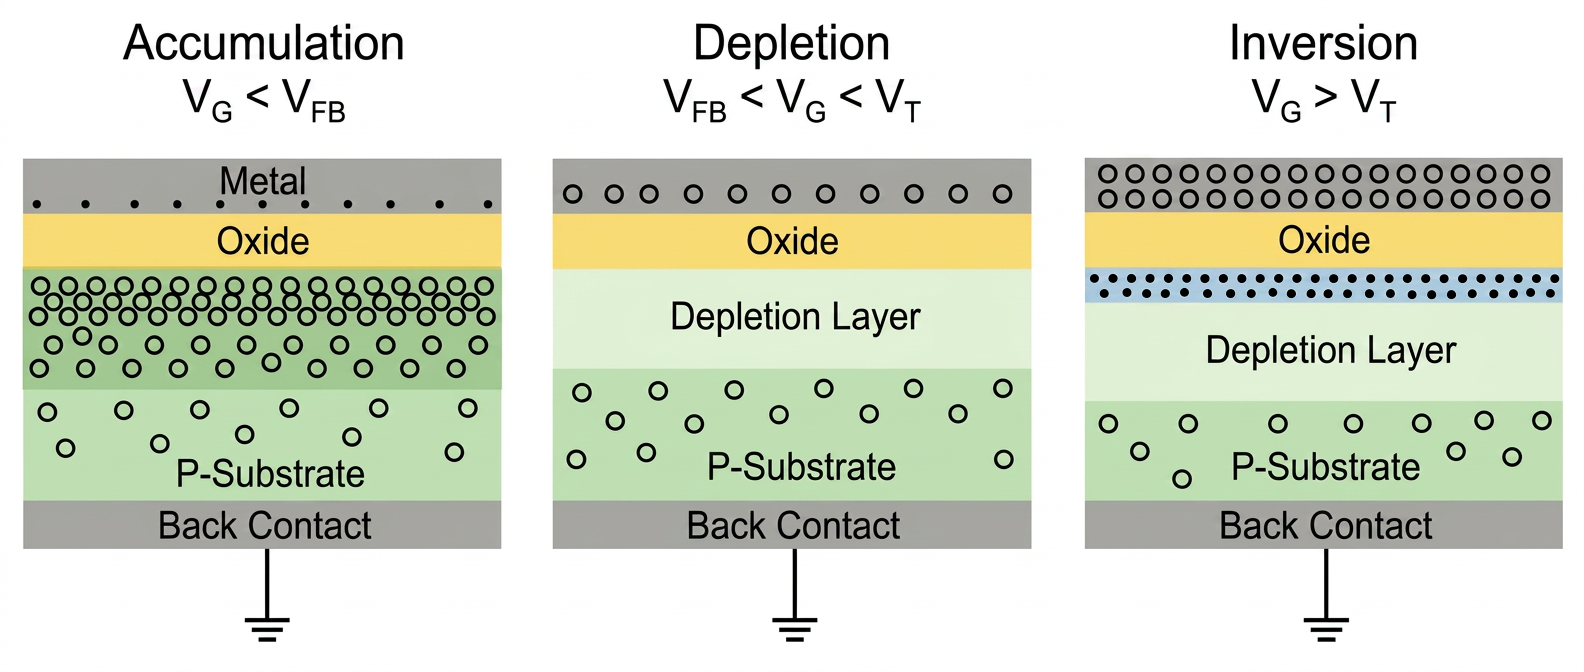
\includegraphics[width=0.72\linewidth]{mos.png}

  \vspace{0.4em}
  \scriptsize 连续电压和电流最终要落到真实器件行为上

  \column{0.50\linewidth}
  \small
  \begin{itemize}
    \item 真实电路处理的是连续电压、电流、延迟与噪声
    \item 数字设计把它组织成离散的 0 / 1 与受控的状态更新
    \item 这层抽象成立的前提不是“世界本来就数字化”
    \item 而是：\textbf{电平可分、噪声可容、延迟可控、边界明确}
  \end{itemize}

  \vspace{0.4em}
  \textbf{后面的 VTC、setup/hold、metastability，都是在保护这层抽象。}
\end{columns}
\end{frame}

\begin{frame}{N-Type and P-Type Materials: Device Background}
\begin{columns}[T]
  \column{0.48\linewidth}
  \centering
  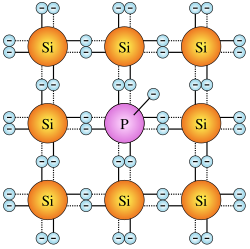
\includegraphics[width=0.78\linewidth]{n-type.png}

  \vspace{0.3em}
  \scriptsize N 型材料：常见示意为掺杂磷，电子是主要载流子

  \column{0.48\linewidth}
  \centering
  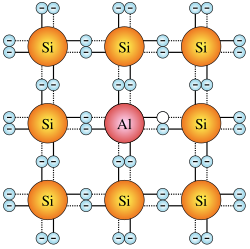
\includegraphics[width=0.78\linewidth]{p-type.png}

  \vspace{0.3em}
  \scriptsize P 型材料：常见示意为掺杂铝，空穴是主要载流子
\end{columns}

\vspace{0.5em}
\small
这些材料直觉本身还不是 NMOS / PMOS，但它们提供了后续 MOS 器件形成沟道与控制导通路径的物理背景。
\end{frame}

\begin{frame}{Pull-Up / Pull-Down Networks}
\begin{columns}[T]
  \column{0.46\linewidth}
  \centering
  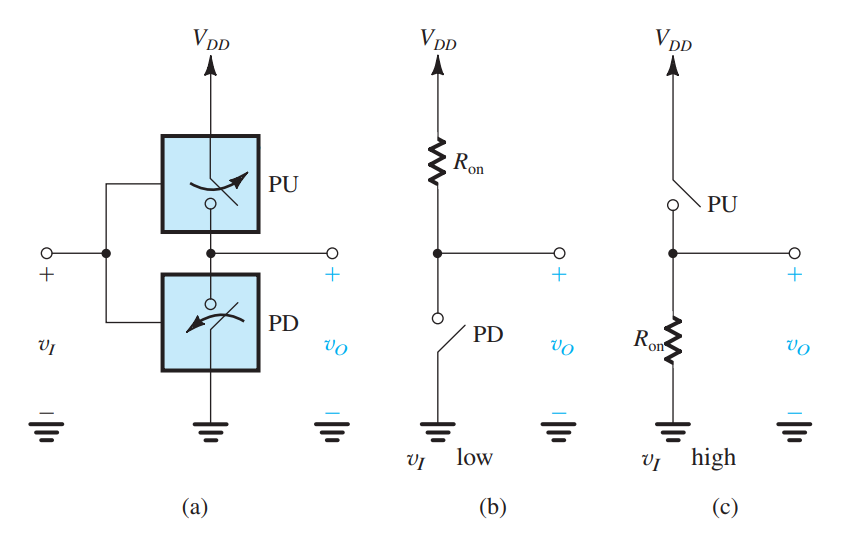
\includegraphics[width=0.86\linewidth]{pu_pd.png}
  \column{0.50\linewidth}
  \small
  \begin{itemize}
    \item PMOS 组成 \textbf{pull-up network}，把输出拉向 \texttt{VDD}
    \item NMOS 组成 \textbf{pull-down network}，把输出拉向 \texttt{GND}
    \item 静态 CMOS 的核心要求：正常情况下两张网络互补工作
    \item 目标不是“永远有电流流动”，而是让输出稳定停在高或低
  \end{itemize}

  \vspace{0.4em}
  \textbf{门电路不是符号游戏，而是导通路径的组织问题。}
\end{columns}
\end{frame}

\begin{frame}{The Inverter: Smallest Complete Digital Gate}
\begin{columns}[T]
  \column{0.50\linewidth}
  \centering
  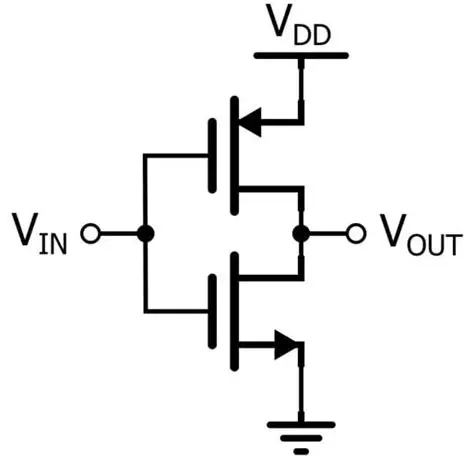
\includegraphics[width=0.92\linewidth]{inverter.png}
  \column{0.45\linewidth}
  \small
  \begin{itemize}
    \item 输入低：PMOS 导通、NMOS 关断，输出被上拉为 1
    \item 输入高：NMOS 导通、PMOS 关断，输出被下拉为 0
    \item 它把“输入控制导通路径”转换成“输出翻转”
    \item 反相器之所以基础，是因为它同时最简单、最规则、通常也最快
  \end{itemize}
\end{columns}
\end{frame}

\begin{frame}{VTC, Noise Margin, and Why 0/1 Are Reliable}
\begin{columns}[T]
  \column{0.50\linewidth}
  \centering
  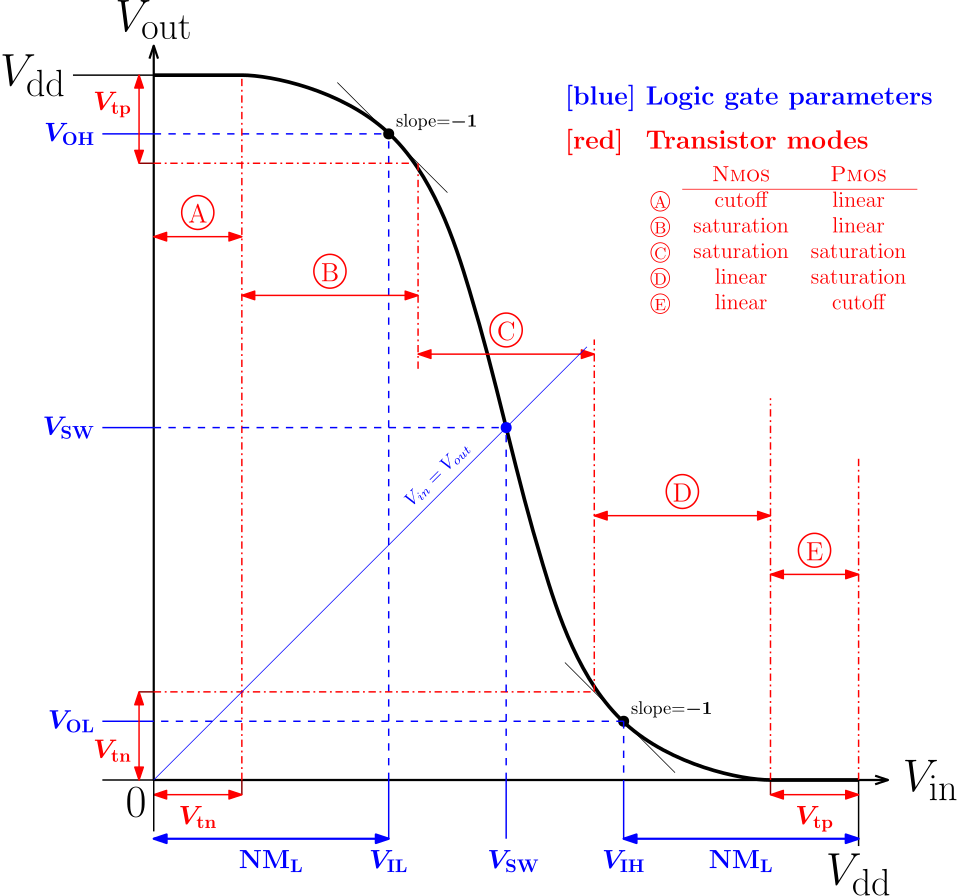
\includegraphics[width=0.92\linewidth]{vtc.png}
  \column{0.45\linewidth}
  \small
  \begin{itemize}
    \item 电压传输特性（VTC）展示输入变化如何映射到输出变化
    \item 两端平台区给出稳定逻辑区间，中间陡峭区是翻转区
    \item \textbf{噪声容限} 的作用：允许信号带着扰动仍被正确识别为 0 或 1
    \item 数字抽象依赖的不是完美电平，而是足够宽的可判别区间
  \end{itemize}
\end{columns}
\end{frame}

\begin{frame}{Delay Comes From Real Devices}
\begin{columns}[T]
  \column{0.44\linewidth}
  \centering
  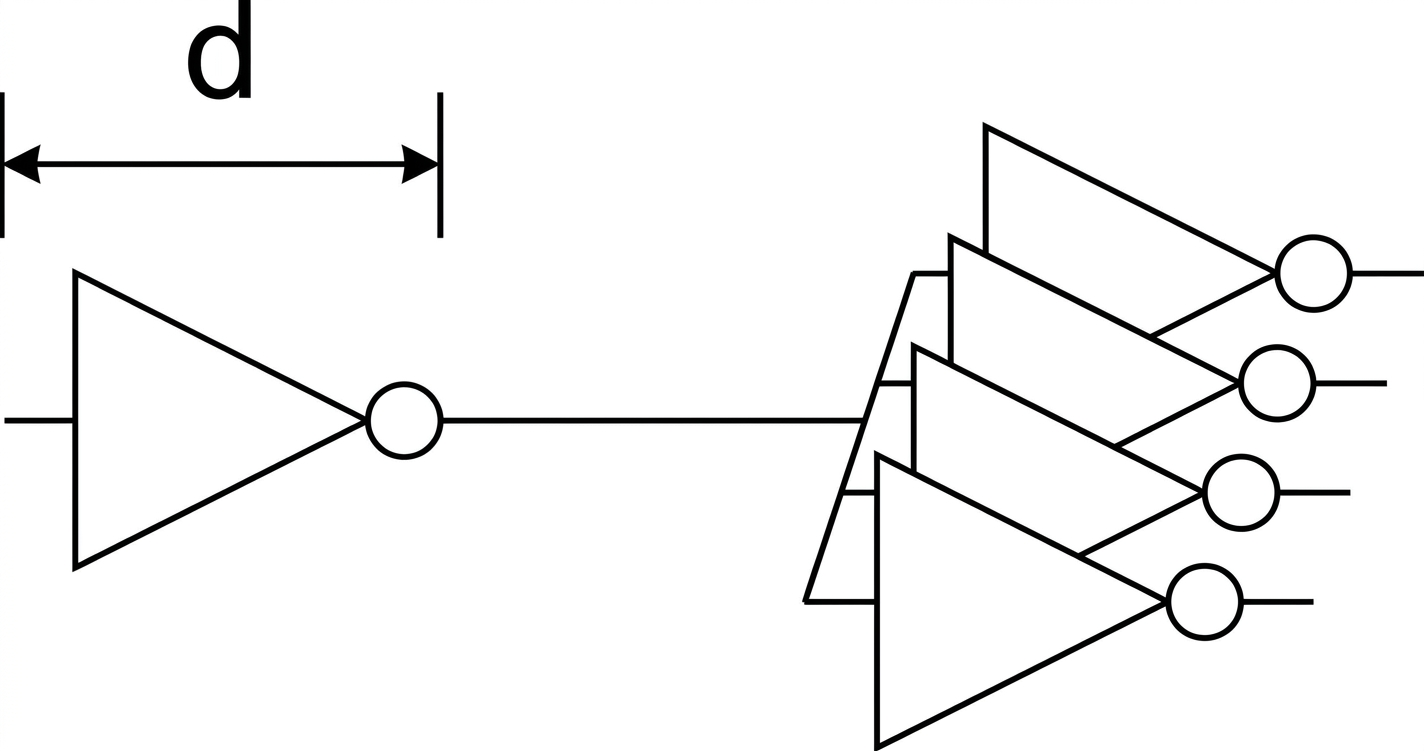
\includegraphics[width=0.44\linewidth]{fo4.png}

  \vspace{0.3em}
  \scriptsize FO4：常用标准延迟参考

  \column{0.52\linewidth}
  \small
  \begin{itemize}
    \item 输出翻转要经历电容充电 / 放电，不可能瞬时完成
    \item 输入边沿越慢、负载越重、扇出越大，门延迟通常越大
    \item 上升沿和下降沿也未必对称
    \item 输入翻转区间内，PMOS/NMOS 可能短时间同时导通，出现短路电流
  \end{itemize}

  \vspace{0.4em}
  \textbf{结论：门延迟不是静态常数，而是上下文相关的。}
\end{columns}
\end{frame}

\begin{frame}{Ring Oscillator: Delay Is Not a Footnote}
\begin{columns}[T]
  \column{0.48\linewidth}
  \centering
  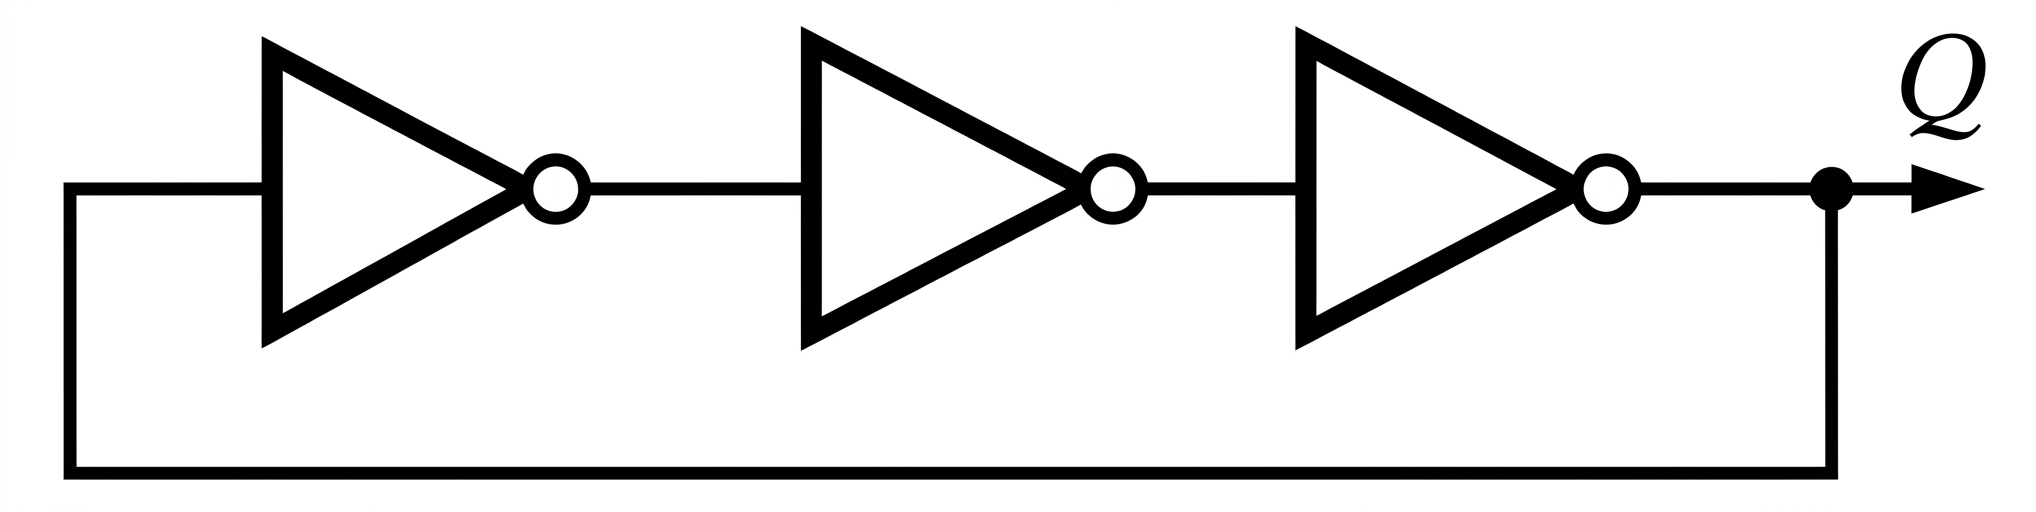
\includegraphics[width=0.90\linewidth]{ring.jpeg}
  \column{0.48\linewidth}
  \small
  \begin{itemize}
    \item 奇数个反相器首尾相接，不会收敛到静态值
    \item 信号会沿着反相链不断传播并翻转
    \item 振荡周期直接受每级延迟影响
    \item 这说明“延迟”不是实现细节，它会直接决定系统行为
  \end{itemize}

  \vspace{0.5em}
  \textbf{如果忽略延迟，就解释不了为什么它会振。}
\end{columns}
\end{frame}

\begin{frame}{From Inverter to NAND / NOR}
\begin{columns}[T]
  \column{0.58\linewidth}
  \centering
  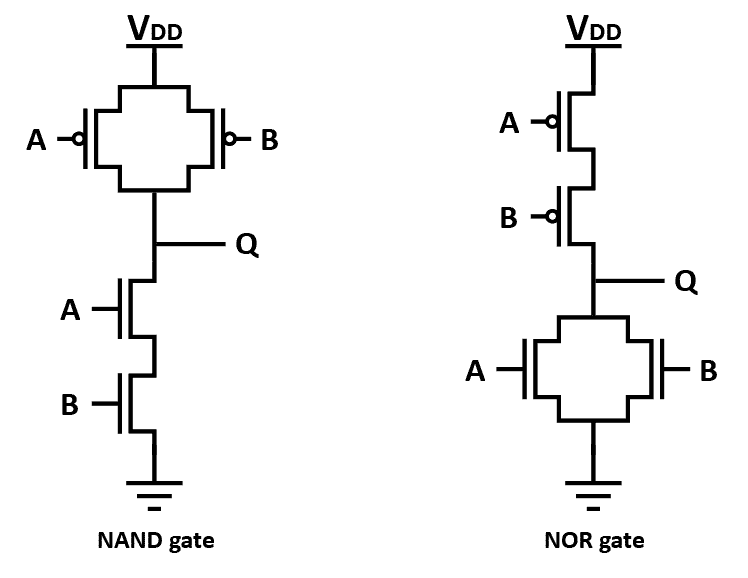
\includegraphics[width=0.48\linewidth]{nand-nor-schema.png}
  \column{0.37\linewidth}
  \small
  \begin{itemize}
    \item NMOS 串联更适合表达 AND 条件下的下拉
    \item PMOS 并联更适合表达 OR 条件下的上拉
    \item 互补地组织两张网络，就得到静态 CMOS NAND / NOR
    \item 真值表、布尔表达式与晶体管结构是三种互相可翻译的视角
  \end{itemize}
\end{columns}
\end{frame}

\begin{frame}{Gate Symbol, Layout View, and Standard Cell Intuition}
\begin{columns}[T]
  \column{0.32\linewidth}
  \centering
  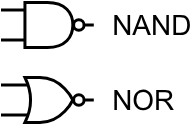
\includegraphics[width=0.95\linewidth]{nand-nor-symbol.png}

  \vspace{0.3em}
  \scriptsize 逻辑符号视角

  \column{0.32\linewidth}
  \centering
  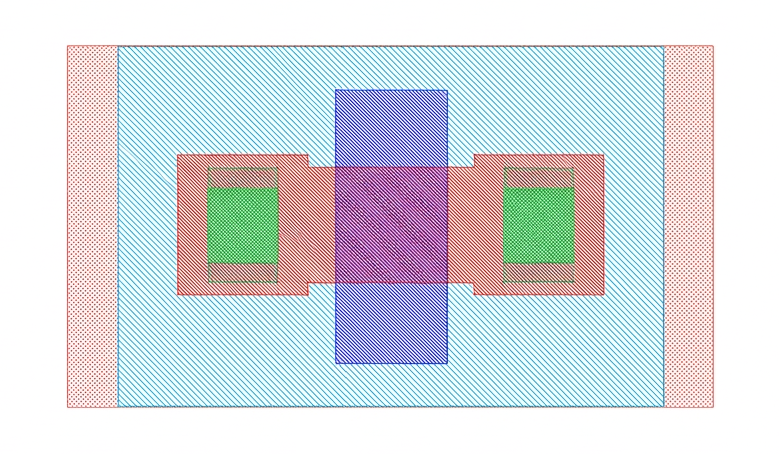
\includegraphics[width=0.95\linewidth]{nmos_layout.png}

  \vspace{0.3em}
  \scriptsize 器件 / 版图视角

  \column{0.32\linewidth}
  \centering
  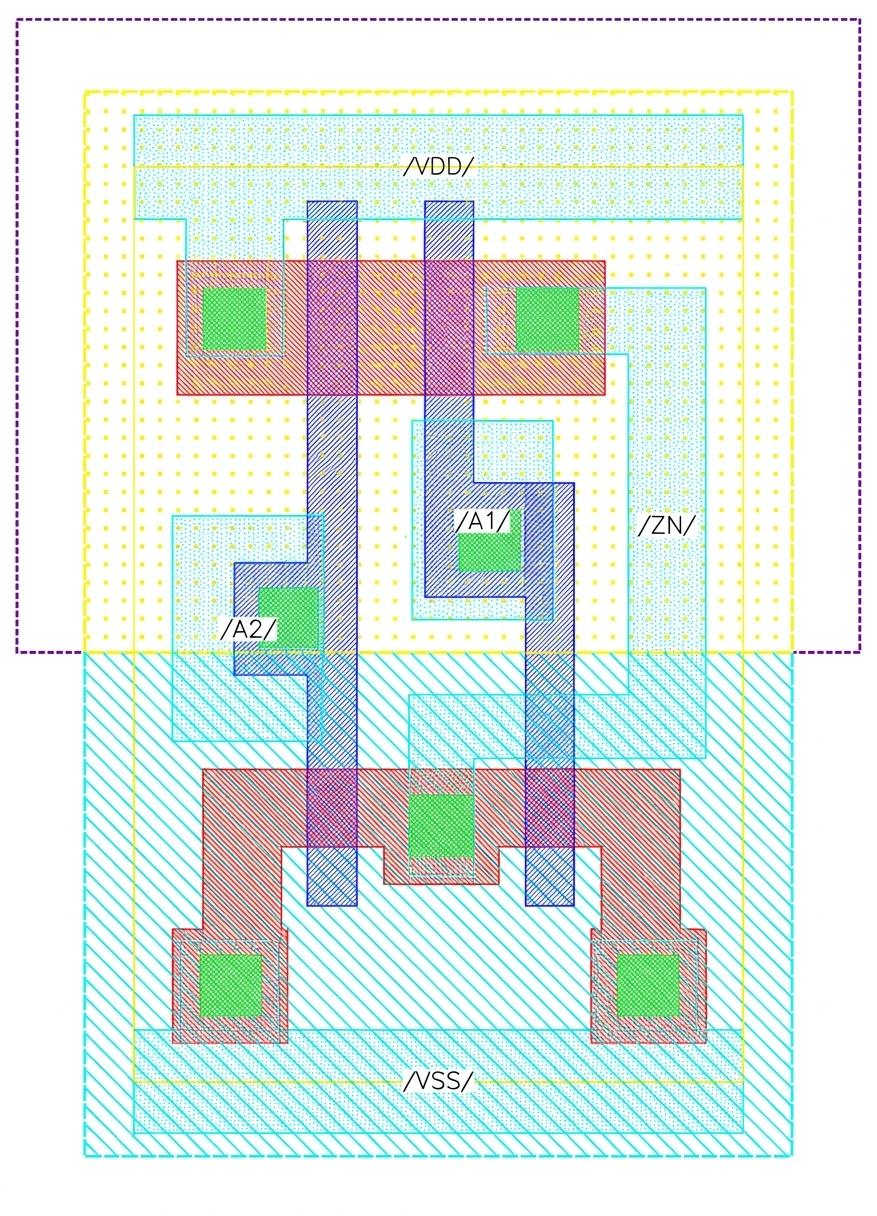
\includegraphics[width=0.95\linewidth]{nor_layout.jpeg}

  \vspace{0.3em}
  \scriptsize 规则化单元视角
\end{columns}

\vspace{0.5em}
\small
逻辑门最后会落成有边界、有引脚、有面积和速度权衡的物理对象。\texttt{AOI/OAI}、不同 drive strength 的单元都属于这条线的延伸。
\end{frame}

\begin{frame}{Combinational Logic Is a Current-Input / Current-Output Mapping}
\begin{columns}[T]
  \column{0.48\linewidth}
  \centering
  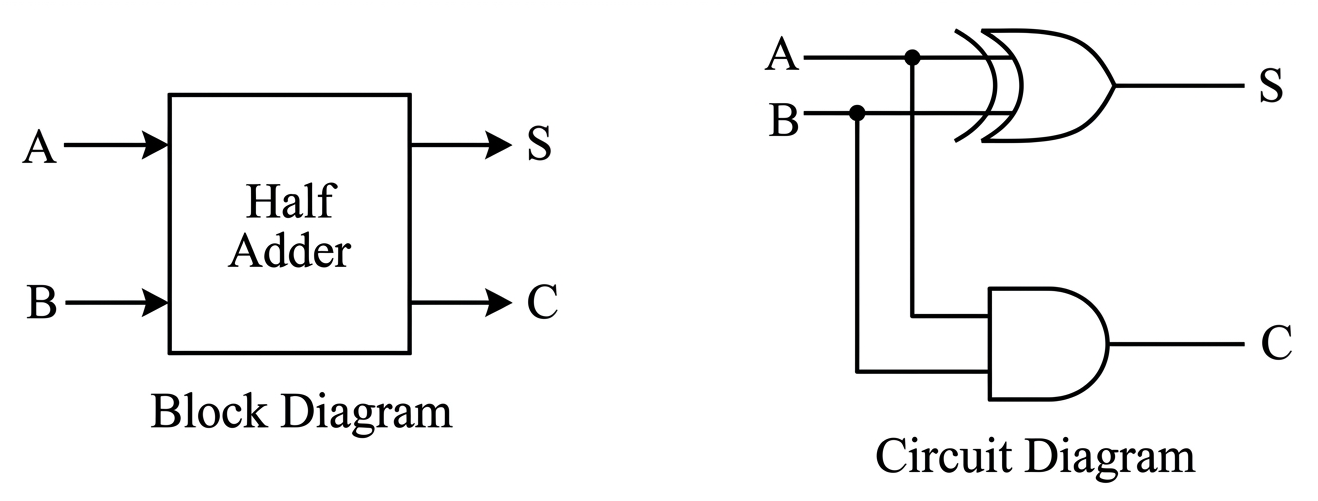
\includegraphics[width=0.90\linewidth]{half_adder.png}
  \column{0.48\linewidth}
  \small
  \begin{itemize}
    \item 组合逻辑的定义：\textbf{当前输出只依赖当前输入}
    \item 半加器把两个输入映射成 \texttt{SUM} 和 \texttt{CARRY}
    \item 你可以在真值表、表达式和门级结构之间往返切换
    \item 全加器、译码器、比较器，都是同一组织方式的扩展
  \end{itemize}
\end{columns}
\end{frame}

\begin{frame}{Hazard and Glitch: Why Combinational Logic Still Has Time Trouble}
\begin{columns}[T]
  \column{0.50\linewidth}
  \centering
  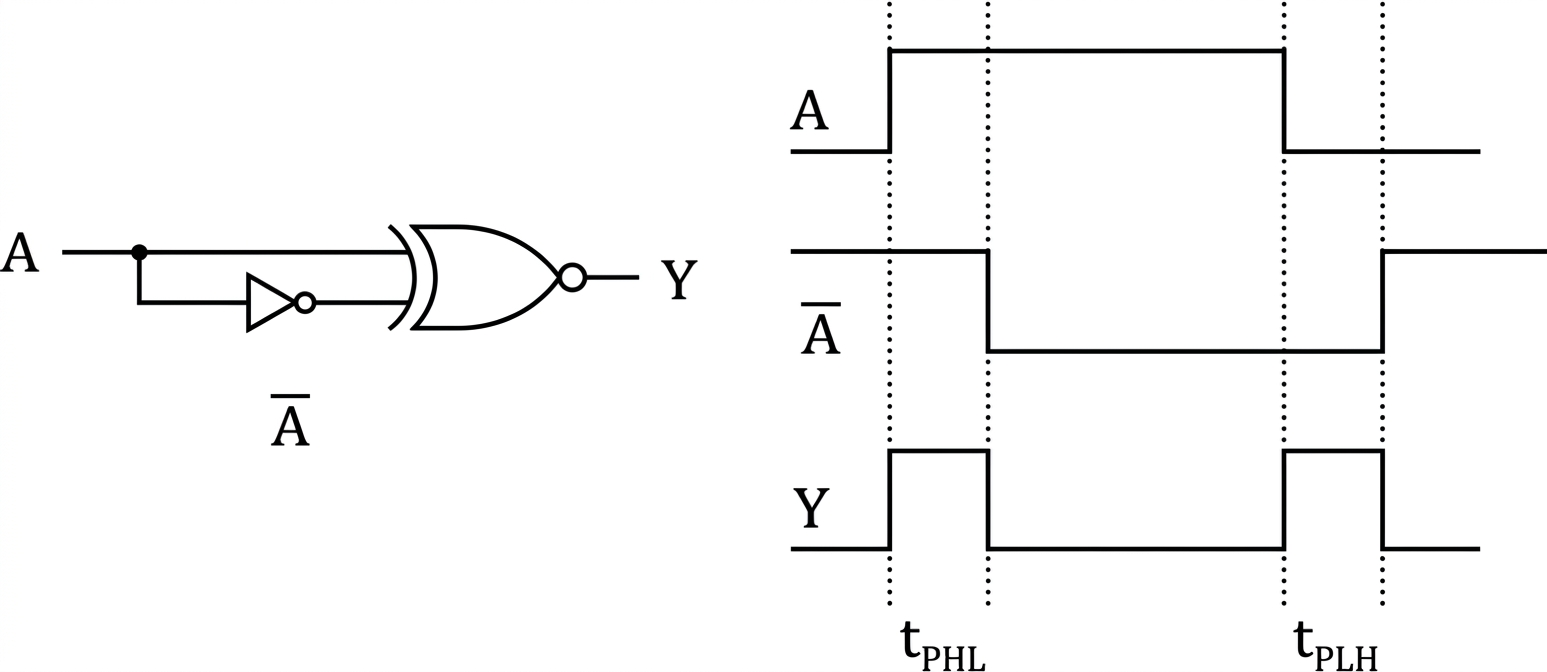
\includegraphics[width=0.92\linewidth]{race_hazard.jpeg}
  \column{0.46\linewidth}
  \small
  \begin{itemize}
    \item 逻辑上等价，不代表时间上同时到达
    \item 不同路径延迟不同，就可能在输出端短暂出现毛刺
    \item 这类问题常被叫做竞争（race）与冒险（hazard）
    \item 如果毛刺被后级寄存器或异步接口看到，它就不再是“无害瞬态”
  \end{itemize}

  \vspace{0.4em}
  \textbf{所以“功能正确”与“时间上安全”不是同一个命题。}
\end{columns}
\end{frame}

\begin{frame}{A Small Reminder: Static CMOS Is Not the Only Way}
\begin{columns}[T]
  \column{0.46\linewidth}
  \centering
  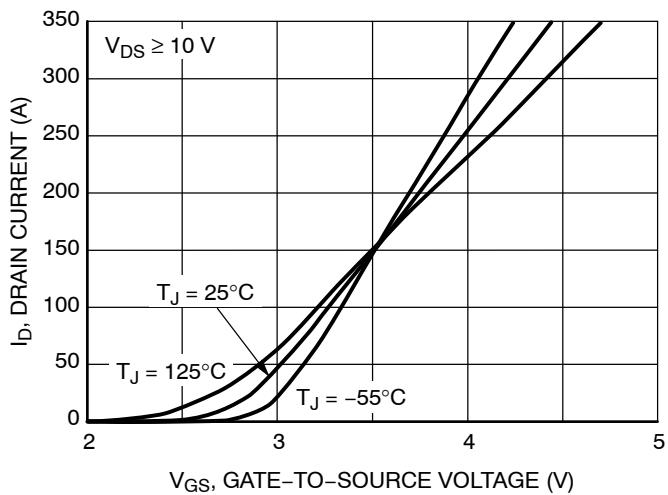
\includegraphics[width=0.82\linewidth]{transfer.jpg}
  \column{0.50\linewidth}
  \small
  \begin{itemize}
    \item 传输门提醒我们：数字逻辑不只靠静态 CMOS 门组织
    \item 它常用于开关、复用、锁存器等结构里
    \item 这一讲只建立“存在其他组织方式”的视野
    \item 重点仍然放在最稳固的主线：器件 $\rightarrow$ 反相器 $\rightarrow$ 基础逻辑门 $\rightarrow$ 组合逻辑
  \end{itemize}
\end{columns}
\end{frame}

\begin{frame}{Takeaways}
\begin{itemize}
  \item 数字抽象成立，是因为真实器件能把电压范围组织成可判别、可恢复的逻辑电平
  \item CMOS 反相器是最小完整基元，NAND / NOR 则把这种组织方式推广成可组合的逻辑门
  \item 门延迟、fanout、transition 与竞争/冒险说明：时间问题并不是后端才出现
  \item 下一讲的寄存器、setup/hold 与 metastability，本质上是在继续保护这层抽象
\end{itemize}
\end{frame}

\begin{frame}{After-Class Prompt}
请完成三件事：
\begin{enumerate}
  \item 画出 CMOS 反相器，分别标出输入为 0 和 1 时的导通路径
  \item 根据半加器真值表写出 \texttt{SUM} 与 \texttt{CARRY} 的表达式，并画出门级结构
  \item 观察一个两条路径延迟不同的组合逻辑网络，解释毛刺为什么出现
\end{enumerate}
\end{frame}

\end{document}
